\documentclass[a4paper,10pt]{article}
\usepackage{amsmath}
\usepackage{amsfonts}
\usepackage{multicol}
\usepackage{{graphicx}}
\usepackage[margin=0.3in]{geometry}

\setlength\parindent{0pt}

\begin{document}
\begin{multicols}{2}
\textbf{Multiplication and permutation rules}\\
sample k is drawn from a population of n distinc objects:\\
Order doesn't matter and replace: $C_{n+k-1}^{k}$ \\
Order doesn't matter and no replace: $C_n^k$

\textbf{Probability Axioms}\\
$P(A\bigcup B\bigcup C)=P(A)+(B)+P(C)-P(A\bigcap B)-P(A\bigcap C)-P(B\bigcap C)+P(A\bigcap B\bigcap C)$\\
Conditional probability: $P(B|A)=P(A\bigcap B)/P(A)$\\
Independent events: two events are independent if: 1) $P(A|B)=P(A)$; 2) $P(B|A)=P(B)$; 3) $P(A\bigcap B)=P(A)P(B)$

\textbf{Bayes theorem \& Conditional probabilities}\\
$P(A|B)=P(B|A)P(A)/P(B)$

\textbf{Discrete Distribution}
\textit{mean}: measure of center of mass; 1st moment; $\mu=E(X)=\sum_x x*P(X=x)$\\
\textit{variance}: measure of dispersion; 2nd moment; $\sigma^2=V(X)=\sum_x(x-\mu)^2f(x)=E(x^2)-\mu^2$ (can be infinite: $P(X=x)\ge 1/x^3$)\\
\textit{skewness}: how asymmetric is the distribution around the mean. Normalized 3-rd moment: $\gamma=E((x-\mu)^3/\sigma^3)$ (can be infinite: $P(X=x)\ge 1/x^4$)\\
\textit{geometirc mean}: for very broad distribution. Mean is dominated by very unlikely but very large events (like lottery). It is $exp(E(logX))$. \\
\textbf{NOTE}: All can be infinite.

\textbf{Discrete uniform distribution}\\
$f(x)=1/(b-a+1)$, a, b is integer. $\mu=(b+a)/2$, $\sigma^2=[(b-a+1)^2-1]/12$

\textbf{Bernouli distribution}\\
$f(x)=p,if\ x=1;1-p,if\ x=0$. $E(X)=p; Var(X)=p(1-p)$

\textbf{Binomial distribution}\\
Sum of n independent bernouli trials, $f(x)=C_x^np^x(1-p)^{n-x}$. $E(X)=np;Var(X)=np(1-p)$

\textbf{Poisson distribution}\\
$P(x)=\cfrac{\lambda^xe^{-\lambda}}{x!}$. $E(X)=Var(X)=\lambda$
\begin{itemize}
\item covered genome fraction: $coverage=\lambda=NL/G; P(X>0)=1-exp(-\lambda);G_{covered}=G*P(X>0)$
\item how many configs: modified $\lambda=(N-1)(L-L_{ov}/G)$, probability no left ends fall inside a read, $N_{config}=Nexp(-\lambda)$
\item average length of config: $G_{covered}/N_{config}$
\end{itemize}

\textbf{Geometric distribution}\\
continue until success: $P(X=x)=p(1-p)^{x-1}$.
$E(X)=1/p;Var(X)=(1-p)/p^2$\\
Example: time to last common maternal ancestor: $P(T=t)=(1-1/N)^{t-1}(1/N)$

\textbf{Negative binomial distribution}
number of trials until r successes: $f(x)=C_{r-1}^{x-1}p^r(1-p)^{x-r}$. $E(X)=r/p;Var(X)=r(1-p)/p^2$\\
Example: cancer passenger and driver mutation

\textbf{Power Law Distribution}\\
$P(X=x)=Cx^{-\lambda}$, where C is normlization term, $1=\sum_xC.x^{-\lambda}$ -> $C=1/\zeta(\lambda)$. Mean and variance can be infinite. \\
Example: protein-protein network; cancer mutation

\textbf{Continuous Distribution}\\
PDF is the derivative of CDF: $f(x)=\cfrac{dF(x)}{dx}$.
$E(X)=\int_{-\infty}^\infty xf(x)dx;Var(X)=\int_{-\infty}^\infty x^2f(x)dx-\mu^2$

\textbf{Contunous uniform distribution}\\
$f(x)=1/(b-a)$. $E(X)=(b+a)/2;Var(X)=(b-a)^2/12$

\textbf{Constant rate (poisson process)}\\
Discrete events happen at rate $r$; expected \#events in time $x$ is $rx$. The actual \#events $N_x$ is a poisson distribution discrete random variable. $p(N_x=n)=\cfrac{(rx)^n}{n!}exp(-rx)$. $E(N_x)=pL=rx$

\textbf{Exponential Distribution}\\
Models the time interval to the 1st event. Exponential random variable X describes \textbf{interval} between 2 successes of a constant rate random process with success rate r per unit interval.
\begin{itemize}
    \item PDF: $f(x)=re^{-rx}, 0\le x<\infty$
    \item CCDF: $P_x(X>x)=P_N(N_x=0)=exp(-rx)$
    \item $u=E(X)=\cfrac{1}{r}$ and $\sigma^2=V(X)=\cfrac{1}{r^2}$
\end{itemize}
\textbf{the only memoryless distribution}: $P(x>t+s|x>s)=P(x>t)$

\textbf{Erlang Distribution}\\
Models the time interval to the $k^{th}$ event, a sum of k exponentially distributed variables.\\
$P(X>x)=\sum_{m=0}^{k-1}\cfrac{e^{-rx}(rx)^m}{m!}=1-F(x)$\\
$f(x)=F(x)'=\cfrac{r^kx^{k-1}e^{-rx}}{(k-1)!}$

\textbf{Gamma Distribution}\\
random variable x with PDF as $f(x)=\cfrac{r^kx^{k-1}e^{-rx}}{\Gamma(k)}$ has a gamma random distribution. If k is an positive integer, X has an Erlang distribution.\\
$\int_0^{\infty}f(x)dx=1 \rightarrow \Gamma(k)=\int_{0}^{\infty}r^k x^{k-1}e^{-rx}dx=\int_0^{\infty}y^{k-1}e^{-y}dy,\ where\ y=rx$

Properties of Gamma function:
\begin{itemize}
    \item $\Gamma(1)=1$
    \item $\Gamma(k)=(k-1)\Gamma(k-1)$, recursive property
    \item $\Gamma(k)=(k-1)!$, factorial function
    \item $\Gamma(1/2)=\pi^{1/2}=1.77$
\end{itemize}
Mean and Variance of Erlang and Gamma:
$\mu=E(X)=k/r$, $\sigma^2=V(x)=k/r^2$

\textbf{Normal/Gaussian Distribution}\\
$f(x)=\cfrac{1}{\sqrt{2\pi}\sigma}e^{\cfrac{-(x-\mu)^2}{2\sigma^2}}\sim N(\mu,\sigma)$
The sum of many independent random variables could be approximated with a Gaussian.

Standard Normal Distribution: $Z\sim N(0, 1)$. CDF is $\Phi(z)=P(Z\le z)$\\
$N\sim(\mu,\sigma)$ can be \textbf{standardized} into $N\sim(0,1)$ by $Z=\cfrac{X-\mu}{\sigma}\rightarrow P(X\le x)=P(Z\le z)$

\textbf{Lognormal Distribution}\\
$X=e^W$, where $W~N(\theta,\omega)\rightarrow W=ln(X)$
$X$ is a lognoraml distribution variable. 
$F(x)=P(X<x)=P(exp(W)\le x)=P(W\le ln(x))=P(Z\le \cfrac{ln(x)-\theta}{\omega})=\Phi(\cfrac{ln(x)-\theta}{\omega})$ for $x>0$; or 0 if $x\le 0$\\
$f(x)=\cfrac{dF(x)}{dx}=\cfrac{1}{x}\cfrac{1}{\omega\sqrt{2\pi}}exp(-(\cfrac{ln(x)-\theta}{2\omega})^2)$ for $x>0$\\
$E(X)=e^{\theta+\omega^2/2}$ and $V(X)=e^{2\theta+\omega^2}(e^{\omega^2}-1)$

\textbf{Joint Probability Distribution}\\
Joint PMF, $f_{XY}(x,y)$\\
Marginal probability distribution: 1) $f_X(x)=\sum_yf_{XY}(x,y)$; 2) $f_Y(y)=\sum_xf_{XY}(x,y)$\\
Use marginal distributions to compute E and V:
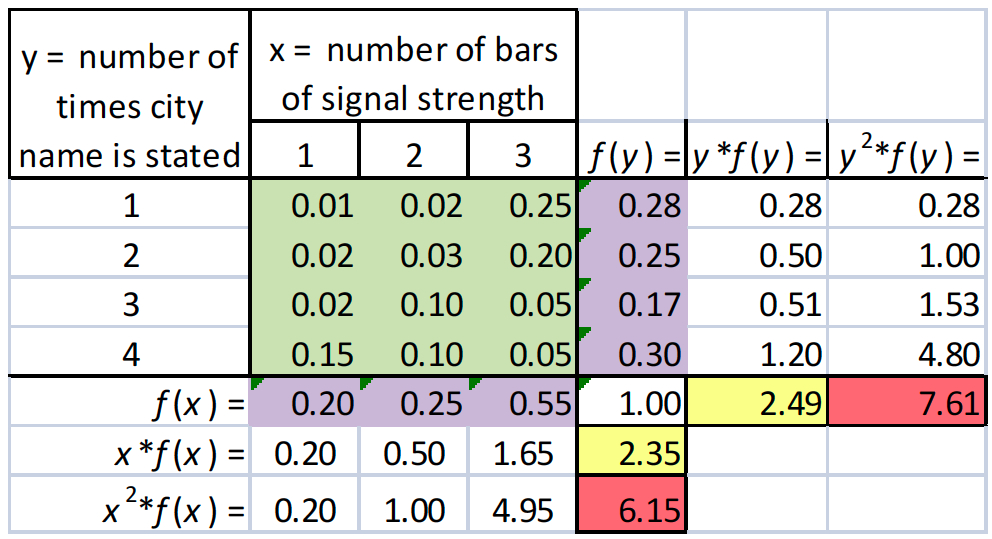
\includegraphics[width=0.4\textwidth]{joint_pd.jpg}

$E(X)=2.35;V(X)=6.15-2.35^2$
$E(Y)=2.49;V(X)=7.61-2.49^2$

Conditional probability distribution: 
$P(Y=y|X=x)=P(X=x,Y=y)/P(X=x)=f(x,y)/f_X(x)$

Random variables independent if all events A that Y=y and B that X=x are independent if any one of the conditions is met:\\
\begin{itemize}
    \item $P(Y=y|X=x)=P(Y=y)$
    \item $P(X=x|Y=y)=P(X=x)$
    \item $P(X=x,Y=y)=P(X=x)P(Y=y)$ for every pair of x and 
\end{itemize}

Conditional probability density function: $f_{Y|x}(y)=\cfrac{f_{XY}(x,y)}{f_X(x)}$\\
Independence of continuous random variable:
\begin{itemize}
\item $f_{XY}(x,y)=f_X(x)f_Y(y)$
\item $f_{Y|x}(y)=f_Y(y); f_{X|y}=f_X(x)$
\item $P(X\subset A,y\subset B)=P(X\subset A)P(Y\subset B)$
\end{itemize}

\textbf{Covariance \& Correlation}
\textbf{Covariance}: measure dependence between random varibales\\
$Cov(X,Y)=\delta_{XY}=E(XY)-\mu_X\mu_Y\in (-\infty,\infty)$
If independent, $Cov(X,Y)=0$. $\rho_{XY}=0$ is necessary for independence, but not sufficient. 

\textbf{Correlation}: \\
Pearson correlation: normalized covariance to test linear relationship between X and Y, unlikely for broad distribution.
$\rho_{XY}=\sigma_{XY}/\sigma_X\sigma_Y\in [-1,1]$

Spearman rank correlation: test monotonic relationship between X and Y. 
Calculate ranks (1 to n), $r_X(i)$ and $r_Y(i)$, $Spearman(X,Y)=Pearson(r_X,r_Y)$

\textbf{Linear functions of random variables}\\
$Y=c_1X_1+c_2X_2+...+C_pX_p$\\
$E(Y)=c_1E(X_1)+...+c_pE(X_p)$\\
$V(Y)=c_1^2V(X_1)+c_p^2V(X_p)+2\sum_{i<j}\sum c_ic_jcov(X_iX_j)$\\
If $cov(x_i,x_j)=0\rightarrow V(Y)=c_1^2V(X_1)+...+c_p^2V(X_p)$

Average of X: $\overline X=(X_1+X_2+..X_p)/p$, then $E(\overline X)=\mu;V(\overline X)=\delta^2/p$

\end{multicols}

\textbf{Appendix}\\
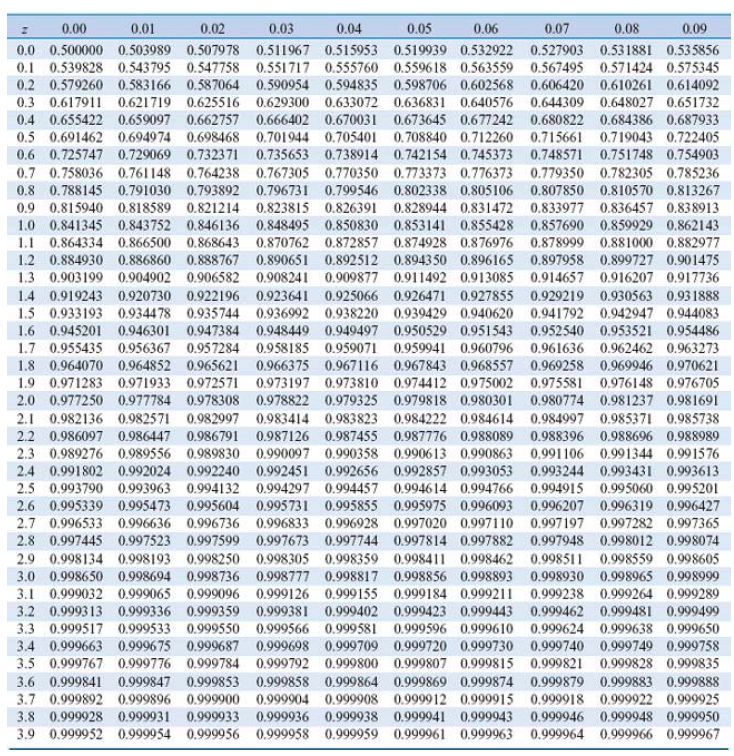
\includegraphics[width=0.8\textwidth]{norm_table.png}

\end{document}